\documentclass[11pt]{article}
\usepackage{setspace}  % To use linespacing
\usepackage{indentfirst} % Indents first line after sections
\usepackage{amssymb} % For \mathbb
\usepackage{enumerate} % For changing labels of enumerate
\usepackage[margin=1in]{geometry} % For editing margins
\usepackage{tikz} % Tikz drawing for graphs
\usetikzlibrary{arrows.meta} % Allows customizing arrows

\usepackage{amsmath}

% Make new commands
\newcommand{\N}{\mathbb{N}}
\newcommand{\R}{\mathbb{R}}
\newcommand{\Z}{\mathbb{Z}}
\newcommand{\abs}[1]{\left|#1\right|}
\newcommand{\fivespace}{\space\space\space\space\space}

% Start main document
\begin{document}
\onehalfspacing
\hfill Frank Cline

\hfill Math 307

\hfill HW 4

% Sections
% 3.4 # 1, 2, 5, 8, 17
% 3.5 # 2, 4, 5, 8, 12
% 11.1 # 1, 15acd, and look at hw4 pdf for another problem
% 11.2 # look online

% SECTION 3.4 # 1, 2, 5, 8, 17
\section*{3.4}
\begin{enumerate}
\item Which of the following describe equivalence relations? For those that are not equivalence relations, specify which of $(R),(S),(T)$ fail and illustrate the failures with examples.
	\begin{enumerate}
	\item $L_1||L_2$ for straight lines in the plane if $L_1$ and $L_2$ are the same or are parallel.\\
	.
	\item $L_1\perp L_2$ for straight lines in the plane if $L_1$ and $L_2$ are perpendicular.\\
	.
	\item $p_1\sim p_2$ for Americans if $p_1$ and $p_2$ live in the same state.\\
	.
	\item $p_1\approx p_2$ for Americans if $p_1$ and $p_2$ live in the same state or in neighboring 
	states.\\
	.
	\item $p_1\approx p_2$ for people if $p_1$ and $p_2$ have a parent in common.\\
	.
	\item $p_1\cong p_2$ for people if $p_1$ and $p_2$ have the same mother.\\
	.
	\end{enumerate}
\item For each example of an equivalence relation in Exercise 1, describe the members of some equivalence class.
	\begin{enumerate}
	\item  DO WORK HERE
	\end{enumerate}
\setcounter{enumi}{4}
\item If $G$ and $H$ are both graphs with vertex set $\{1,2,...,n\}$, we say that $G$ is isomorphic to $H$, and write $G\cong H$, in case there is a way to label the vertices of $G$ so that it becomes $H$.
\[
	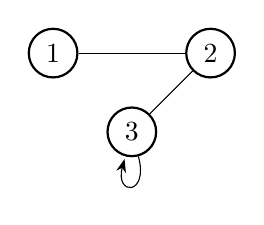
\begin{tikzpicture}
	\begin{scope}[every node/.style={circle,thick,draw}]
	    \node (1) at (0,0) {$1$};
	    \node (2) at (2,0) {$2$};
	    \node (3) at (1,-1) {$3$};
	\end{scope}
	
	\begin{scope}[>={Stealth[black]},
	              every node/.style={fill=white,circle},
	              every edge/.style={draw=black}]
	    	\path (1) edge (2);
	    	\path (2) edge (3);
		\path (3) edge[loop below] (3);
	\end{scope}
	\end{tikzpicture}
	\cong
	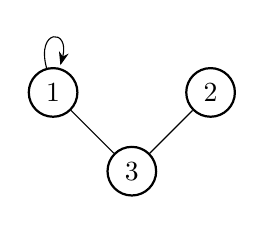
\begin{tikzpicture}
	\begin{scope}[every node/.style={circle,thick,draw}]
	    \node (1) at (0,0) {$1$};
	    \node (2) at (2,0) {$2$};
	    \node (3) at (1,-1) {$3$};
	\end{scope}
	
	\begin{scope}[>={Stealth[black]},
	              every node/.style={fill=white,circle},
	              every edge/.style={draw=black}]
	    	\path (1) edge[loop above] (1);
	    	\path (1) edge (3);
		\path (3) edge (2);
	\end{scope}
	\end{tikzpicture}
\]
	\begin{enumerate}
	\item Give a picture of another graph isomorphic to these two.\\
	.
	\item Find a graph with vertex set $\{1,2,3\}$ that is not isomorphic to the graphs yet has three edges and exactly one is 
	a loop.\\
	.
	\item Find another example as in part(b) that isn't isomorphic to the answer of part(b) and the other two graphs.\\
	.
	\item Show that $\cong$ is an equivalence relation on the set of all graphs with the vertex set $\{1,2,...,n\}$.\\
	.
	\end{enumerate}
\setcounter{enumi}{7}
\item
	\begin{enumerate}
	\item For $m,n\in\Z$, define $m\sim n$ in case $m-n$ is odd. Is the relation reflexive? symmetric? transitive? Is it an 
	equivalence relation?\\
	.
	\item For $a$ and $b$ in $\R$, define $a\sim b$ in case $a-b\leq 1$. One could say that $a\sim b$ in case $a$ and $b$ are 
	close enough or approximately equal. Answer the question in part (a).\\
	.
	\end{enumerate}
\setcounter{enumi}{16}
\item 
	\begin{enumerate}
	\item Verify that the relation $\cong$ defined in Example 5b (the reachable Relation $R$ on $V(G)$ by $(v,w)\in R$) is an 
	equivalence relation on $V(G)$.\\
	.
	\item Given a vertex $v$ in $V(G)$, describe in words the equivalence class containing $v$.\\
	.
	\end{enumerate}

\end{enumerate}


\end{document}